\documentclass{beamer}
%Information to be included in the title page:
% Language setting
% Replace `english' with e.g. `spanish' to change the document language
\usepackage[english]{babel}
\usepackage{csquotes}
% Useful packages
\usepackage{amsmath}
\usepackage{graphicx}
\usepackage{hyperref}

\usepackage{biblatex} %Imports biblatex package
\addbibresource{motivation.bib}
\addbibresource{cryo-em.bib}
\addbibresource{ensembles.bib}


\title{Intrinsically Disordered Proteins}

\subtitle{Extending the Model of Proteins to Account for Disorder}

\author{Maeve Andersen}


\date{Autumn Semester, 2023}


\begin{document}

\frame{\titlepage}

\begin{frame}
\frametitle{Introduction}
In 1894, Fischer developed a protein model to describe the biological function of proteins. In this model, the protein acts as a key of sorts, where the protein's unique shape determines its unique biological function (the lock) \cite{fischerEinflussConfigurationAuf1894}.
\end{frame}
\begin{frame}
\frametitle{Introduction}
This is the so called "lock and key model" which depends on proteins having rigid 3D structure \cite{fischerEinflussConfigurationAuf1894}.
\end{frame}

\begin{frame}
\frametitle{Introduction}
Today however, protein scientists have found a class of proteins that have no rigid structure, yet play a key role in many biological functions. This class of proteins are called "intrinsically disordered proteins" or proteins having disorder. Disussion of how protein disorder is modeled will be the subject of this talk.
\end{frame}

\begin{frame}
\frametitle{Motivation}
Characterization of disorder in proteins is important as disordered proteins are involved in cellular signaling and regulation,\cite{wrightIntrinsicallyDisorderedProteins2015}
and are associated with human diseases, such as neurodegenerative disease, cardiovascular disease, amyloidoses, cancer, and diabetes.\cite{uverskyIntrinsicallyDisorderedProteins2008}
Although challenging, modern methods of characterizing proteins can provide new insights to crucial protein function human biological mechanisms. \cite{bonomiSimultaneousDeterminationProtein2018}.
\end{frame}

\begin{frame}
\frametitle{The "Outline" of Protein Structure Determination}
Todo make a diagram of how proteins are determined
\end{frame}

\begin{frame}
\frametitle{Energy Landscapes}
\begin{figure}[h]
    \centering
    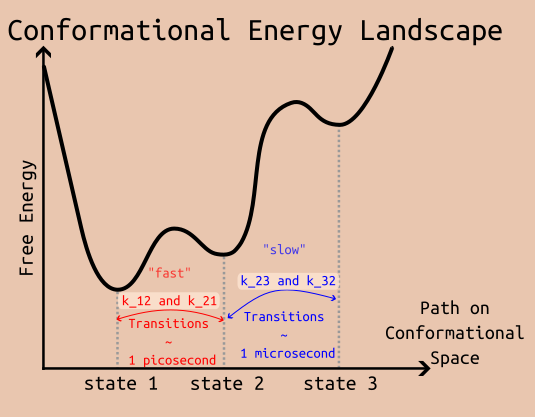
\includegraphics[scale=0.55]{energy-landscape.png}
    \caption{Transition rates and the protein's energy landscape.
        Low populated states often switch "slow" on a time scale of millisecons.
    Highly populated states often switch "fast" on the time scale of picoseconds \cite{bonomiDeterminationProteinStructural2019}. }
    \label{fig:min-bacteria}
\end{figure}
%Transition rates are the kinematics of the protein.
%Dynamics are based on the kinemetics. 

\end{frame}
\begin{frame}
\frametitle{Forward Models}
TODO: insert forward model description of RCD as example
\end{frame}

\begin{frame}
    \frametitle{Bayesian Weighting}
TODO introduce baysian weighting
\end{frame}


\begin{frame}
\frametitle{Aside: Flexible Meccano example}
Todo
\end{frame}

\begin{frame}
    \frametitle{Bayesian Weighting Cont.}
Todo wrap up description of Bayesian Weighting by talking about how degeneracy occures with Flexible Meccano
\end{frame}
\begin{frame}
    \frametitle{Perspectives on Protein Science}
    Below are perspectives on disordered proteins taken from various review papers:
    \begin{itemize}
        \item More robust/transferrable representations of structural ensembles \cite{bonomiDeterminationProteinStructural2019}
        \item Well defined threshold of "acceptable" results/accessible ways of comparing ensembles \cite{bonomiDeterminationProteinStructural2019}
        \item More transferrable and accurate force fields to help with integrative methods \cite{thomasenConformationalEnsemblesIntrinsically2022}
        \item Unified forward models: Developing forward models that are transferrable between proteins that do and do not have disorder \cite{thomasenConformationalEnsemblesIntrinsically2022}
    \end{itemize}
\end{frame}

\begin{frame}
    \frametitle{Conclusion}
    In this talk I reviewed the current state of protein science regarding how to handle disorder in proteins.
    Disorder is a many dimensional problem, which has necessitated the use of rigourous methods that combine computation with experiment.
    This has led to many interesting sub problems such as how to handle degeneracy and how to deal with the and quantification of errors.
    Most importantly though, the recent work done to characterize proteins may lead to many practical applications in treating human disease.

\end{frame}

\begin{frame}
\frametitle{References}
\printbibliography

\end{frame}

\begin{frame}
    \frametitle{Thank you to:} 
    \begin{itemize}
        \item Kevin Stenson: for supporting me over the summer and during this semester
        \item My girlfriends: Beth, Rae, June, and Maya: for emotionally supporting me through this time of rapid change
        \item My parents, Sherry and Rob: for making this "try" financially possible
        \item The queer and disabled community: for giving me a foundation of understanding for who I am
    \end{itemize}
\end{frame}

\end{document}
